\documentclass[conference]{IEEEtran}

%I have 5 1/2 pages, have 2 1/2 left

%3/4 2-way (PCR included), 3/4 A-PEQ,  = 1 1/2, maybe 1 page?
% 1/2 theoremas (without proof)
% 1 page simulations
% total 3 pages - need to shrink 1/2 page.
 
%(pretty close)

% outline
%
% S and F for guaranteed rate servers
%
% Introduce the issue of fairness and what we want to do with fairness
%
%
% Briefly introduce the EQ server,
%         then introduce as a subsection the packetized scheduling
%               review the delay theorem as in ICON 2013
%
% Introduce Efficient Attempt (issues, overview etc)
%
% Introduce the two-way scheduler
%
%    a) The two scheduler principle, define it, show picture
%    b) Define the top scheduler as VC2 (mention it messes up delay)
%    c) mention the issues in the bottom scheduler, why it cannot be simply
%       fair queuing, and why we have to do something else.
%
% Introduce A-PEQ, 
%
%   mention that we do a round-robin scheduler, which is fed whever there is
%   no one at A
%
%
%   Mention the unfairness problem, and the need for delta
%
%
%   Present the scheduler itself
%
%
% Delay bound
%
%   Simple theorem on delay bound 
%
% Experimental Results.





%\documentclass{article}
\usepackage{amsmath}
\usepackage{graphicx}
%\usepackage{epsfig}
\usepackage{epic}
\usepackage{eepic}
\usepackage{eepicemu}
\usepackage{color}

%\usepackage{latexsym}
%\setlength{\textwidth}{7in}
%\setlength{\textheight}{9in}
%\setlength{\headheight}{-.5in}
%\addtolength{\oddsidemargin}{-1in}
%\addtolength{\evensidemargin}{-1in}

%%%%%%%%%%%%%%%%%%%%%%%%%%%%%%%%%%%%%%%%%%%%%%%%%%%%%%%%%%%%%%%%%%%%%%%%%%%%%%%%%
%
%            Lyx list environment.
%
%%%%%%%%%%%%%%%%%%%%%%%%%%%%%%%%%%%%%%%%%%%%%%%%%%%%%%%%%%%%%%%%%%%%%%%%%%%%%%%%%
 \newenvironment{lyxlist}[1]
   {\begin{list}{}
     {\settowidth{\labelwidth}{#1}
      \setlength{\leftmargin}{\labelwidth}
      \addtolength{\leftmargin}{\labelsep}
      \renewcommand{\makelabel}[1]{##1\hfil}}}
   {\end{list}}

%%%%%%%%%%%%%%%%%%%%%%%%%%%%%%%%%%%%%%%%%%%%%%%%%%%%%%%%%%%%%%%%%%%%%%%%%%%%%%%%%
%
%                      TABS \,\land\, BOXES
%
%%%%%%%%%%%%%%%%%%%%%%%%%%%%%%%%%%%%%%%%%%%%%%%%%%%%%%%%%%%%%%%%%%%%%%%%%%%%%%%%%
\newcommand{\fatbox}{\\[3pt]\framebox(4,14){}}
\newcommand{\qed}{\rule{1.5mm}{1.5mm}}
\newcommand{\QED}{\rule{1.5mm}{1.5mm}}

\newlength{\tabsize}
\setlength{\tabsize}{0.35in}
\newcommand{\settabs}{
\tab{\tabsize}\=\tab{\tabsize}\=\tab{\tabsize}\=\tab{\tabsize}\=\tab{\tabsize}\=\tab{\tabsize}\=\tab{\tabsize}\=\tab{\tabsize}\=\tab{\tabsize}\=\tab{\tabsize}\=\tab{\tabsize}\=\tab{\tabsize}\=\tab{\tabsize}\=\kill
}
\newcommand{\tabbox}{\makebox[\tabsize]{\ }}

\newcommand{\tea}{\>}
\newcommand{\teb}{\>\>}
\newcommand{\tec}{\>\>\>}
\newcommand{\ted}{\>\>\>\>}
\newcommand{\tee}{\>\>\>\>\>}
\newcommand{\tef}{\>\>\>\>\>\>}
\newcommand{\teg}{\>\>\>\>\>\>\>}
\newcommand{\teh}{\>\>\>\>\>\>\>\>}
\newcommand{\tei}{\>\>\>\>\>\>\>\>\>}
\newcommand{\tej}{\>\>\>\>\>\>\>\>\>\>}
\newcommand{\tek}{\>\>\>\>\>\>\>\>\>\>\>}

\newcommand{\tab}[1]{\makebox[#1]{}}

\newtheorem{theorem}{Theorem}
\newtheorem{lemma}{Lemma}
\newtheorem{corollary}{Corollary}
\newtheorem{definition}{Definition}
\newenvironment{proof}{{\scshape Proof: }}{\hfill\qed}


%%%%%%%%%%%%%%%%%%%%%%%%%%%%%%%%%%%%%%%%%%%%%%%%%%%%%%%%%%%%%%%%%%%%%%%%%%%%%%%
%
%                      MISC
%
%%%%%%%%%%%%%%%%%%%%%%%%%%%%%%%%%%%%%%%%%%%%%%%%%%%%%%%%%%%%%%%%%%%%%%%%%%%%%%%
\newcommand{\CP}{\prime}
\newcommand{\CPP}{{\prime\prime}}
\newcommand{\guard}{\langle\mbox{\sf guard}\rangle}
\newcommand{\assignment}{\langle\mbox{\sf assignment}\rangle}
\newcommand{\guardCP}{\langle\mbox{\sf guard}^\CP\rangle}
\newcommand{\assignmentCP}{\langle\mbox{\sf assignment}^\CP\rangle}


%\newcommand{\vect}[1]{{#1}v}
%\newcommand{\vect}[1]{\vec{#1}}

%\newcommand{\shadow}[1]{\widehat{#1}}
%\newcommand{\shadow}[1]{#1^*}

\begin{document}

\title{An Approximation to Rate-Equalization Fairness with Logarithmic 
Complexity for QoS}
\author{\authorblockN{Jorge A. Cobb \ \ \ \ \ \ Suparn Gupta}
\authorblockA{Department of Computer Science\\
The University of Texas at Dallas\\
Richardson, TX 75083-068875080-3021\\
Email: \{cobb,\ suparn.gupta\}@utdallas.edu}
}

\maketitle

\begin{abstract}
Scheduling protocols that provide both rate and fairness guarantees, such as 
Weighted Fair Queuing, distribute the unused capacity among the flows in 
proportion to the reserved rate of the flows. Thus, flows whose reserved 
rate is the largest will receive a larger share of the unused capacity. In 
earlier work, we have presented a scheduling algorithm that first 
distributes unused capacity to those flows whose reserved rate is the least.  
However, the per-packet complexity of this algorithm, known as 
rate-equalization (REQ) fairness, is linear in the number of flows. In this 
paper, we present an algorithm that approximates the behavior of REQ 
fairness but with only logarithmic complexity per packet. Simulation results 
show that in practical situations the behavior of the approximation 
algorithm is quite similar to that of pure REQ fairness.
\smallskip\\
{\em Keywords:} Quality of Service Scheduling, Real-Time Traffic, Fairness in 
Bandwidth Allocation.
\end{abstract}

%\maketitle

\newcommand{\femph}[1]{{#1}^{*}}



%%%%%%%%%%%%%%%%%%%%%%%%%%%%%%%%%%%%%%%%%%%%%%%%%%%%%%%%%%
%
\section{Introduction}
%
%%%%%%%%%%%%%%%%%%%%%%%%%%%%%%%%%%%%%%%%%%%%%%%%%%%%%%%%%
%The need for QoS schedulers in the Internet, Intserv
{\em While the best effort service provided by the Internet suffices for 
traditional applications, such as email and web browsing, real-time 
applications such as interactive audio and video require Quality of Service 
(QoS)
guarantees from the network. In particular, they require the network to reserve bandwidth for the application and to provide a bounded end-to-end delay. To provide these QoS guarantees, a broad array of packet
scheduling protocols have been developed, such as Virtual Clock (VC) \cite{VC-Lam, VC-Lixia} and Weighted Fair Queuing (WFQ) \cite{GPS-Parekh}. These and many others belong to a large family of scheduling protocols, known as rate-guaranteed schedulers \cite{Cobb-Flow-Theory-ToN,leaveintime,NOSSDAV-95-Vin} which provide a guaranteed end-to-end delay bound.


%Need for fairness
One desirable property of a rate-guaranteed scheduler is fairness. That is, a flow should not be ``punished'' (temporarily denied service) if it exceeds its reserved rate to take advantage of unused bandwidth in the channel. Some protocols, such as Virtual Clock, are unfair, while others, like WFQ, are fair. 

%from TS ToN
The fairness property is desirable because it may be normal for some flows to violate their reserved packet rate. Examples of such flows are file transfers and multi-resolution video \cite{hopbyhop}. The sources of these flows will likely  reserve from the network the smallest packet rate necessary to receive a minimum quality of service. If the source detects that additional bandwidth is available, it generates packets at a rate higher than its reserved rate. If the source detects that no additional bandwidth is available, it reduces its sending rate. There are several techniques by which a source can detect if additional bandwidth is available, see for example \cite{Packet-Pair} and \cite{DecBit}. Thus, because some flows may be of adjustable rate, the unused bandwidth of a channel should be shared in a fair manner among all flows.

%Most protocols provide fairness in some way

Most scheduling protocols that provide both rate and fairness guarantees, such as WFQ and its variants \cite{GPS-Parekh} \cite{Hui-Hierarchical-WFQ} \cite{Cobb-TS-Scheduling-ToN} \cite{SCFQ-Golestani} \cite{Hui-WF2Q}, distribute the unused capacity among the flows in proportion to the reserved rate of the flows. Thus, if flow $f$ reserved twice the rate as flow $g$, then $f$'s share of the unused bandwidth is twice that of $g$. 

In this paper, we present an alternative approach for fairness in 
rate-guaranteed schedulers. Our scheduling algorithm first distributes unused 
capacity to those flows whose reserved rate is the least. This allocation 
continues until the flows with least reserved rate and the flows with the 
next-to-least reserved rate are given the same capacity. This continues, level 
by level, until, if enough unused capacity is available, all flows will receive 
the same capacity, and the scheduler will simply behave like Fair Queuing.
}

%%%%%%%%%%%%%%%%%%%%%%%%%%%%%%%%%%%%%%%%%%%%%%%%%%%%%%%%%%%%%%%%%%%%%%%%%
%
\section{QoS Model}
\label{sec:QoS-Model}
%
%%%%%%%%%%%%%%%%%%%%%%%%%%%%%%%%%%%%%%%%%%%%%%%%%%%%%%%%%%%%%%%%%%%%%%%%%%

Our QoS model is based on the models of \cite{Cobb-Flow-Theory-ToN} and 
\cite{leaveintime}. A {\em network} is a set of computers connected via 
point-to-point communication channels. A {\em flow} is a sequence of packets, 
all of which originate at the same source computer and are destined to the 
same computer. All packets of a flow must traverse the network along a fixed 
path. 

Each flow is characterized by its data rate and an upper bound on its 
end-to-end delay. Before a source introduces a new flow to the network, enough 
network resources are reserved to ensure the flow's delay bound is not 
violated. If enough resources are not available, the flow is rejected. 

\begin{figure}[tb]
\centering
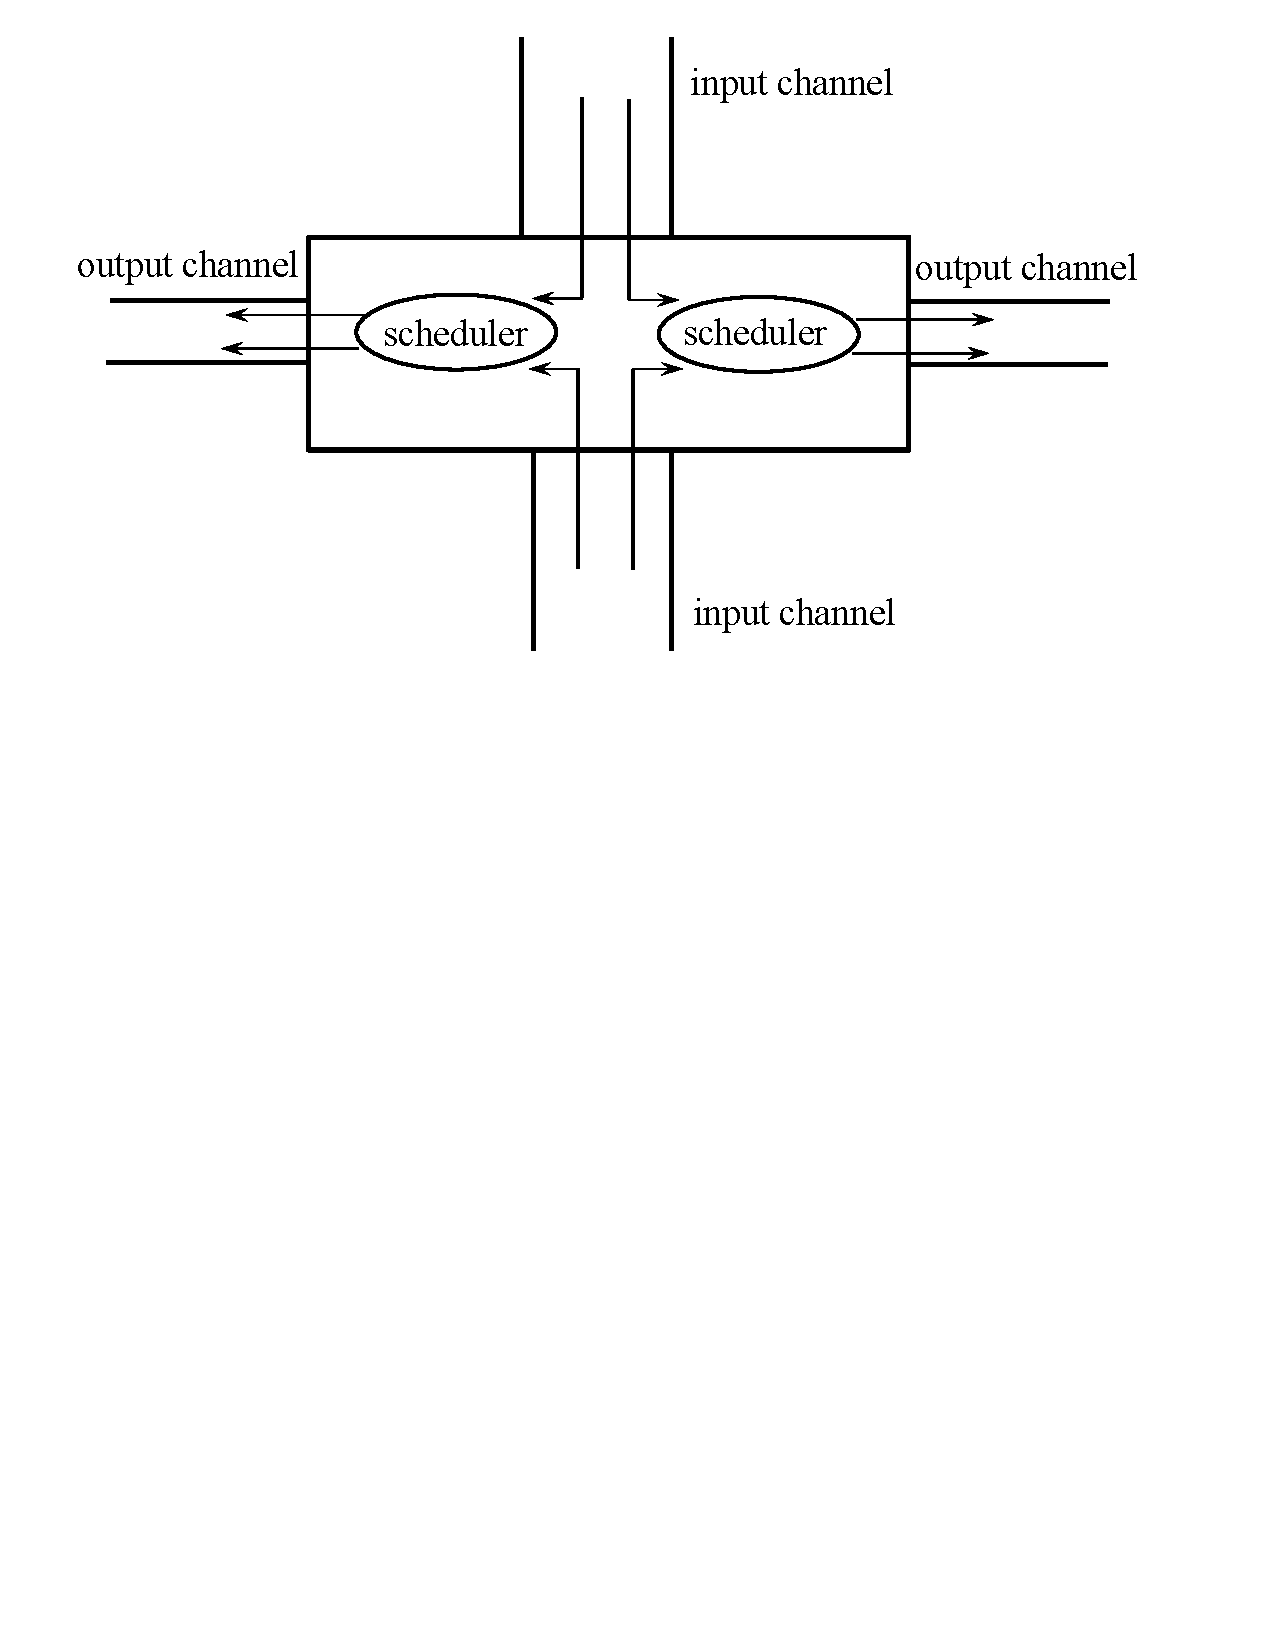
\includegraphics[width=\columnwidth,trim=0in 6.5in 0 0,clip,scale=0.50]{Fig1.pdf}
\caption{Schedulers and Channels}
\label{fig:CobbFig1}
\end{figure}

Each output channel of a computer is equipped with a packet scheduler (see 
Figure \ref{fig:CobbFig1}).  A scheduler receives packets from flows whose path 
traverses its output channel.  Whenever its output channel becomes idle, the 
scheduler chooses a received packet and forwards it over the output channel. A 
packet {\em exits} a scheduler when its last bit packet is transmitted by the 
output channel.  We adopt the following notation for each flow $f$.

\begin{center}
\begin{tabular}{rl}
$R_{f}$ & data rate reserved for flow $f$.
\\
$p_{f,i}$ & $i^{th}$ packet of $f$, $i \geq 1$.
\\
$L_{f,i}$ & length of packet $p_{f,i}$.
\\
$L^{max}_{f}$ & maximum packet length of $f$. 
\\
$L^{max}$ & maximum packet length of all flows.
\\
$A_{f,i}$ & arrival time of $p_{f,i}$.
\\
$E_{f,i}$ & exit time of $p_{f,i}$.
\\
$C$ & bandwidth of the output channel.
\end{tabular}
\end{center}


\begin{figure}
\noindent
\rule{\columnwidth}{0.5mm}
\centerline{\bf CR Server}
\begin{tabbing}
\settabs
let $B(t)$ be the set of backlogged flows at time $t$;\\
for every flow $f$, \\
\tea if $f \in B(t)$, then\\
\teb     $\psi_{f,CR}(t) = R_f$\\
\tea else\\
\teb     $\psi_{f,CR}(t) = 0$
\end{tabbing}
\caption{Constant-rate fluid server}
\label{fig:CR}
\rule{\columnwidth}{0.5mm}
\end{figure}

Consider a constant-rate (CR) fluid server\footnote{Fluid servers can forward, 
during any time interval, an arbitray number of bits from any subset of its 
input flows.  They are for reference only and cannot be implemented. This is in 
contrast to  packet schedulers which are used in practice and can only forward 
one packet at a time.}  whose input is a set of flows, among them $f$.  Let 
this server forward the bits of each input flow $f$ at exactly its reserved 
rate $R_f$.  Such a fluid server is defined in Fig. \ref{fig:CR}, where $B(t)$ 
are the {\em backlogged flows} at time $t$, i.e., flows with bits remaining to 
be forwarded, and $\psi_{f,CR}(t)$ is the bit rate given to flow $f$ at time 
$t$.  

We define $S_{f,i,CR}$ as the {\em start-time} of packet $p_{f,i}$ at the 
constant-rate server and $F_{f,i,CR}$ as the {\em finishing time}.  They can be 
computed recursively as follows, where $S_{f,1,CR} = A_{f,1}$.
\begin{eqnarray}
\nonumber S_{f,i,CR} & = & \mbox{max}(A_{f,i},\ F_{f,i-1,CR})
                 \ \ \mbox{$i > 1$}\\
F_{f,i,CR} & = & S_{f,i,CR} + \frac{L_{f,i}}{R_{f}}
                 \ \ \mbox{$i \geq 1$} \label{eq:F-def}
\end{eqnarray}
Note that $F_{f,i,CR}$ is the value used by the Virtual Clock scheduling 
protocol to assign priorities to its packets \cite{VC-Lam, VC-Lixia}.

Assume that a packet scheduler $s$ forwards the packets of an input flow $f$ at 
a rate of at least $R_f$. Then, each packet $p_{f,i}$ exits scheduler $s$ not 
much later than its finishing time at $CR$, i.e., $F_{f,i,CR}$. We refer to 
these packet schedulers as {\em rate-guaranteed schedulers} 
\cite{Cobb-Flow-Theory-ToN,leaveintime,NOSSDAV-95-Vin}. More formally, a 
scheduler $s$ is a rate-guaranteed scheduler iff, for every input flow $f$ of 
$s$ and every $i$, $i \geq 1$,
\[
E_{f,i,s} \leq F_{f,i,CR} + \delta_{f,s}
\]
for some constant $\delta_{f,s}$. For many protocols, such as Virtual Clock 
\cite{VC-Lam, VC-Lixia} and Weighted Fair Queuing \cite{GPS-Parekh}
(and their many variations),
\[
\delta_{f,s} = L^{max}_s/C_s
\]
I.e., packets exit by their finishing time in $CR$ plus at most the time to 
transmit the largest packet size. In this case, admission control is 
simple\footnote{Other protocols have a {\em rate-independent delay} 
\cite{leaveintime,KGShin94}: where $\delta_{f,s}$ could be negative. This 
allows for a smaller per-hop delay, but makes the admission control test quite 
complex. Such protocols are outside the scope of this paper.
},
the sum of the reserved rates of all the flows through $s$ must be at most $C$.

%The delay of a packet across a sequence of rate-guaranteed schedulers is well 
%known \cite{Cobb-Flow-Theory-ToN,leaveintime,NOSSDAV-95-Vin}, and is simply as 
%follows. Let $t_1, t_2, \ldots , t_k$ be a sequence of $k$ rate-guaranteed 
%schedulers traversed by flow $f$. For all $i$,
%\begin{equation}\label{eq:E-e2e}
%E_{f,i,t_k} \leq  F_{f,i,CR} +
%                  \sum_{x=1}^{k-1} \left( \frac{L^{max}_{f}}{R_{f}} \right) +
%                  \sum_{x=1}^{k} \left(\frac{L^{max}_{t_x}}{C_{t_x}} \right)
%\end{equation}
%Equation (\ref{eq:E-e2e}) is often described as ``paying for bursts only 
%once''. I.e., the burstiness of $f$ affects the exit time $E_{f,i,t_k}$ only 
%by increasing the value of $F_{f,i,CR}$, but it does not affect the per-hop 
%delay of $\frac{L^{max}_{f}}{R_{f}} + \frac{L^{max}_{t_x}}{C_{t_x}}$. 


%%%%%%%%%%%%%%%%%%%%%%%%%%%%%%%%%%%%%%%%%%%%%%%%%%%%%%%%%%%%%
%
\section{Rate-Equalization Fairness}
%
%%%%%%%%%%%%%%%%%%%%%%%%%%%%%%%%%%%%%%%%%%%%%%%%%%%%%%%%%%%%%
\label{sec:Fairness}

We next overview the motivation for rate-equalizing fairness, which we 
introduced in \cite{Cobb-REQ}.

On occasions, the bandwidth of a channel is not fully utilized. This occurs 
either because existing flows are transmitting at a rate that is below their 
reserved rate, or because the sum of the reserved rates of the flows is less 
than the output channel's bandwidth. Under these conditions, it is possible for 
a flow to temporarily exceed its reserved rate, in an attempt to take advantage 
of bandwidth that is not being used by other flows. The source of the flow can 
determine if there is unused bandwidth by receiving implicit feedback from the 
network, in particular, that its packets are experiencing an end-to-end delay 
that is smaller than expected.

The manner in which unallocated bandwidth is distributed among flows varies 
from one scheduling protocol to another. We refer to this distribution of 
unallocated bandwidth as the {\em fairness method} of the protocol, and it is 
the main focus of this paper.

Some protocols, like Virtual Clock (VC) \cite{VC-Lixia}\cite{VC-Lam}, do not 
address fairness. In VC, each packet $p_{f,i}$ is labeled with its virtual 
finishing time, $F_{f,i,CR}$ (see (\ref{eq:F-def})), and packets are forwarded 
by the scheduler in order of increasing labels. A consequence of this is that, 
if a flow exceeds its reserved rate, it may later be denied service by the 
scheduler, for a duration proportional to the time the flow exceeded its rate 
\cite{Cobb-TS-Scheduling-ToN}. This is potentially unbounded. The exit bound in 
Equation \eqref{eq:E-e2e} still holds, however, because VC is a rate-guaranteed 
scheduler.

Other rate-guaranteed protocols, such as Weighted Fair Queuing (WFQ) 
\cite{GPS-Parekh} and its variants  \cite{Hui-Hierarchical-WFQ} 
\cite{Cobb-TS-Scheduling-ToN} \cite{SCFQ-Golestani} \cite{Hui-WF2Q}, distribute 
the unallocated bandwidth among flows in proportion to their reserved rate.  
Specifically, the effective rate $\psi_f$ that is given to flow $f$ (i.e., the 
rate at which the scheduler actually forwards the packets of flow $f$) is
\begin{equation}
\label{eq:WFQ-Share}
\psi_f(t) = \frac{C}{\left(\sum_{g \in B(t)} R_g \right)}\cdot R_f \geq R_f
\end{equation}
where $B(t)$ are the backlogged flows at time $t$ (i.e., those flows with a 
non-empty queue) and $C$ is the capacity of the output channel of the 
scheduler.

Consider another flow $g$ with lesser reserved bandwidth, e.g., $R_f = 2\cdot 
R_g$.  From (\ref{eq:WFQ-Share}), it can be easily shown that
\[
(\psi_f - R_f) = 2\cdot (\psi_g - R_g)
\]
\noindent
That is, the manner in which unused bandwidth is allocated to backlogged flows 
is proportional to the reserved rate of the flow. Hence, the fairness method of 
WFQ favors flows with a higher reserved rate. 

The intuition behind WFQ's fairness method is as follows. If a flow has a 
reserved rate that is greater than that of other flows, it implies that the 
user who generates the flow is paying a greater price for the network service, 
and thus, should receive a greater share of the unallocated bandwidth.

In \cite{Cobb-REQ}, we presented an alternative fairness method in which the 
overall objective is to give every flow the same effective rate, provided 
enough unallocated bandwidth is available. This will result in a value for the 
effective rate $\psi_f$ that is different from the one given in Equation 
\eqref{eq:WFQ-Share}. The intuition behind it is the following. Every flow will 
be guaranteed its reserved rate $R_f$. However, flows whose applications are 
rate-adaptive could reserve the minimum rate possible to satisfy their QoS 
requirements, and thus minimize expense. Any additional bandwidth is given to 
those flows that need it the most, i.e., those with the least reserved rate. 

A more detaied description is as follows. First, at all times, the effective 
rate of any flow $f$, $\psi_f$, is at least its reserved rate, $R_f$. I.e., 
$R_f \leq \psi_f$. Next, consider another flow $g$, where $R_f < R_g$. By 
definition, $R_g \leq \psi_g$.  In our method, if enough unallocated bandwidth 
is available, $\psi_f$ will increase until it becomes equal to $R_g$, and thus, 
$\psi_f$ will become equal to $\psi_g$. Thus, flows with lower reserved rates 
will ``catch up'' to flows with larger reserved rates.

Assume that more unallocated bandwidth remains. In this case, the remaining 
unallocated bandwidth will be distributed equally between $f$ and $g$, 
maintaining the relationship $\psi_f = \psi_g$. If there exists another flow 
$h$, where $R_h > R_g$, then $\psi_f$ and $\psi_g$ increase equally until they 
reach $R_h$ (assuming enough bandwidth remains), and hence, $\psi_f = \psi_g = 
\psi_h$.

To summarize, our fairness method attempts to give all flows the same effective 
rate. However, in doing so, the requirement of $R_f \leq \psi_f$ for all $f$ 
must be preserved at all times.


We next describe our fairness method in a more formal way by introducing a rate 
equalization fluid server, which wll then be emulated as close as possible by a 
packet scheduler.



%%%%%%%%%%%%%%%%%%%%%%%%%%%%%%%%%%%%%%%%%%%%%%%%%%%%%%%%%%%%%
%
\section{Rate-Equalization Server and Scheduler}
%
%%%%%%%%%%%%%%%%%%%%%%%%%%%%%%%%%%%%%%%%%%%%%%%%%%%%%%%%%%%%%

Packet scheduling algorithms that provide fairness, such as WFQ and some of its 
variants, describe their fairness method via a virtual fluid server.  The 
packet scheduler then mimics the fluid server as much as possible. The fluid 
server and the packet scheduler have the same input flows. Both have an output 
channel, and both of these channels have equal capacity.

What distinguishes the fluid server from the packet scheduler is the manner in 
which it forwards bits. Once the packet scheduler begins to transmit a packet, 
the transmission of the packet cannot be preempted. The fluid server, on the 
other hand, can concurrently forward an arbitrary number of bits from a group 
of flows. This, of course, is bounded by the capacity (bits/sec.) of the output 
channel.

%%%%%%%%%%%%%%%%%%%%%%%%%%%%%%%%%%
\subsection{Fluid Server}
%%%%%%%%%%%%%%%%%%%%%%%%%%%%%%%%%%

In light of our earlier discussion on fairness, we define the rate-equalization 
(EQ) fluid server as follows. Let $\psi_{f,EQ}(t)$ be the instantaneous bit 
rate given to flow $f$ by the fluid server. This value is computed as shown in 
Figure \ref{fig:EQ-server}. If $\psi_{f,EQ}(t)$ does not change during an 
interval $[t_1, t_2]$, then the total number of bits of $f$ forwarded during 
this interval is $\psi_{f,EQ}(t_1)\cdot(t_2-t_1)$.

The steps shown in Figure \ref{fig:EQ-server} are as follows. First, the set 
$B(t)$ of backlogged flows (i.e., with bits remaining to be forwarded) is 
determined. Obviously, a non-backlogged flow receives a rate of zero. All other 
flows are then arranged in increasing order of their reserved rate. Then, the 
index $j$ is found such that
\[ R_{b_j} \leq \frac{C - \sum_{k=j+1}^{m}R_{b_k}}{j} < R_{b_{j+1}}
\]
In this manner, if the higher rate flows $b_{j+1}, \ldots , b_{m}$ receive 
exactly their reserved rate, then there is enough remaining bandwidth that can 
be equally shared among the lower rate flows $b_{1}, b_{2}, \ldots , b_{j}$.

\begin{figure}
\noindent
\rule{\columnwidth}{0.5mm}
\centerline{\bf EQ Server}
\begin{tabbing}
\settabs
let $B(t)$ be the set of backlogged flows at time $t$;\\
for every flow $f$, \\
\tea if $f \notin B(t)$, then\\
\teb     $\psi_{f,EQ}(t) = 0$\\
\tea else\\
\teb     let $b_1,b_2,\ldots,b_m$ be the flows of $B(t)$\\
\teb     \ \ ordered by increasing $R$;\\
\teb     let $j$, $1\leq j \leq m$, be the largest index such that\\
\tec          $\displaystyle R_{b_j} \leq
                                 \frac{C - \sum_{k=j+1}^{m}R_{b_k}}{j}
                           < R_{b_{j+1}}$;\\
\teb     let $\displaystyle R_{EQ} = \frac{C - 
\sum_{k=j+1}^{m}R_{b_k}}{j}$;\\
\teb     for each $k$, $1 \leq k \leq j$, \\
\tec          $\psi_{f,EQ}(t) = R_{EQ}$;\\
\teb     for each $k$, $j+1 \leq k \leq m$,\\
\tec          $\psi_{f,EQ}(t) = R_{b_k}$;

\end{tabbing}
\caption{Rate equalization fluid server}
\rule{\columnwidth}{0.5mm}
\label{fig:EQ-server}
\end{figure}




\begin{figure}[t]
\centerline{
\setlength{\unitlength}{0.75in}
\begin{picture}(4,2.6)(-0.25,-0.25)
%(x,y)(x0,y0)  x,y size of box x0y0 coordinate of botton left corner
%axis
\linethickness{1pt}
\put(0,0){\line(1,0){3.5}}
\put(0,0){\line(0,1){2.4}}
\put(0,-0.25){0}
\put(0.95,-0.25){1}
\put(1.95,-0.25){2}
\put(2.95,-0.25){3}
\put(-0.3,0.75){40}
\put(-0.3,1.55){80}
\put(-0.35,2.35){120}
%ticks horizontal
\put(1,0){\line(0,1){0.1}}
\put(1,0){\line(0,-1){0.1}}
\put(2,0){\line(0,1){0.1}}
\put(2,0){\line(0,-1){0.1}}
\put(3,0){\line(0,1){0.1}}
\put(3,0){\line(0,-1){0.1}}
%ticks vertical
\multiput(-0.15,0.2)(0,0.2){12}{
\line(1,0){0.2}
}
%draw lines for the first two seconds
%only three flows
\put(0,0.8){\line(1,0){2}}
\put(0.8,0.4){$\psi_{f_1} = 40$}
%
\put(0,1.6){\line(1,0){2}}
\put(0.8,1.2){$\psi_{f_2} = 40$}
%
\put(0,2.4){\line(1,0){2}}
\put(0.8,2){$\psi_{f_3} = 40$}
%
%dotted line at 2
\linethickness{0.5pt}
\multiput(2,0)(0,0.2){12}{\line(0,1){0.12}}
\linethickness{1pt}
%
%draw lines after the first two seconds
\put(2,0.5){\line(1,0){0.8}}
\put(2.05,0.2){$\psi_{f_1} = 25$}
%
\put(2,1){\line(1,0){0.8}}
\put(2.05,0.7){$\psi_{f_2} = 25$}
%
\put(2,1.6){\line(1,0){0.8}}
\put(2.05,1.25){$\psi_{f_3} = 30$}
%
\put(2,2.4){\line(1,0){0.8}}
\put(2.05,1.95){$\psi_{f_4} = 40$}
%
%dotted line at 2.8
\linethickness{0.5pt}
\multiput(2.8,0)(0,0.2){12}{\line(0,1){0.12}}
\linethickness{1pt}
%
%after 2.8, only three flows
\put(2.8,0.8){\line(1,0){0.7}}
\put(3,0.35){$\psi_{f_2} = 40$}
\put(2.8,1.6){\line(1,0){0.7}}
\put(3,1.15){$\psi_{f_3} = 40$}
\put(2.8,2.4){\line(1,0){0.7}}
\put(3,1.95){$\psi_{f_4} = 40$}
\end{picture}
}
\caption{Fluid server example.}
\label{fig:Fluid-Example}
\end{figure}



Consider the following example, which is illustrated in Fig.
\ref{fig:Fluid-Example}. Let $C = 120$ bits/sec.. There are four flows, $f_1 
\ldots f_4$, and all packets are 100 bits long. Let $R_{f_1} = 10$ bits/sec., 
$R_{f_2} = 20$ bits/sec., $R_{f_3} = 30$ bits/sec., and $R_{f_4} = 40$ 
bits/sec.. Note that $\sum_{i=1}^{4} R_{f_i} = 100$ bits/sec., leaving 20 
bits/sec.  unallocated.

Assume that at time 0, one packet of $f_1$ arrives, two packets of $f_2$ 
arrive, and two packets of $f_3$ arrive. At time 2 secs., one packet of $f_4$ 
arrives.

At time zero, flows $f_1$, $f_2$, and $f_3$ have bits in their queues. Since $C 
= 120$, there is enough capacity for all  three flows to receive the same 
effective bandwidth of $\psi = 40$ bits/sec.. At time 2, a packet from $f_4$ 
arrives.  The total reserved rates of the flows is 100 bits/sec., leaving only 
20 bits/sec. to equalize the rates among the flows. Equalizing $f_1$ to $f_2$ 
requires 10 bits/sec.. The remaining 10 bits/sec. are distributed equally 
between $f_1$ and $f_2$, but are not enough to increase their effective rates 
up $R_{f_3}$. We thus end with $\psi_{f_1} = \psi_{f_2} = 25$ bits/sec. This 
leaves $\psi_{f_3} = R_{f_3} = 30$ bits/sec., and $\psi_{f_4} = R_{f_4} = 40$ 
bits sec.

At time $2\frac{4}{5}$, the last bit of the packet of $f_1$ exits, so only 
three flows have a non-empty queue. Again, all remaining flows are given an 
effective bandwidth of 40 bits/sec.  We leave it to the reader to determine the 
remainder of the example.


%%%%%%%%%%%%%%%%%%%%%%%%%%%%%%%%%%
\subsection{Packet Scheduler}
%%%%%%%%%%%%%%%%%%%%%%%%%%%%%%%%%%


\begin{figure}
\noindent
\rule{\columnwidth}{0.5mm}
\centerline{\bf PEQ Scheduler}
\begin{tabbing}
\settabs
upon receiving a packet $p_{f,i}$,\\
\tea $D_{f,i,PEQ} = \infty$;\\
\\
if output channel is idle at time $t$,\\
\tea model the behavior of $EQ$ up to time $t$;\\
\tea let $p_{f,i} \in \mbox{Active}(t)$ iff $t \geq S_{f,i,EQ}$;\\
\tea for each $p_{f,i} \in \mbox{Active}(t)$,\\
\teb     $D_{f,i,PEQ} = S_{f,i,EQ} + L_{f,i}/R_f$;\\
\tea let $D_{g,j,PEQ} = \mbox{min}\{D_{f,i,PEQ}\,\,|\,\, p_{f,i} \in 
\mbox{Active}(t)\}$;\\
\tea forward $p_{g,j}$ to the output channel.
\end{tabbing}
\caption{Packetized rate equalization scheduler}
\label{fig:PEQ-scheduler}
\rule{\columnwidth}{0.5mm}
\end{figure}


We next overview the packet scheduler for rate-equalization which we presented 
in \cite{Cobb-REQ}, where more details can be found. 

In general, the purpose of a fluid server is to guide the packet scheduler in 
the order it chooses to forward packets. Typically, 
\cite{Cobb-Universal-Timestamp-CN}\cite{GPS-Parekh}\cite{RP-Fair-Servers-ToN}, 
for every pair of packets, $p_1$ and $p_2$, if $p_1$ finishes service in the 
fluid server before $p_2$ finishes service, then the packet scheduler will 
forward $p_1$ before $p_2$. I.e., the packet scheduler tries to emulate the 
behavior of the fluid server as much as possible. This emulation, of course, is 
not perfect, because the packet scheduler can only forward one packet at a 
time, while the fluid server can forward bits of multiple flows (and hence 
multiple packets) at once.

For most fluid servers 
\cite{Cobb-Universal-Timestamp-CN}\cite{GPS-Parekh}\cite{RP-Fair-Servers-ToN}, 
at the moment a packet arrives, the exit time that this packet will have from 
the fluid server is unknown. This is because the bit rate at which the packet 
will be served depends not only on the packets currently in the system, but 
also on packets that are yet to arrive.

In consequence, when a packet $p_{f,i}$ arrives into a packet scheduler, the 
scheduler assigns to the packet a {\em virtual exit time} $T_{f,i}$  (see  
\cite{GPS-Parekh} for details on computing this value), such that, for any 
other packet $p_{g,j}$, $T_{f,i} \leq T_{g,j}$ iff the exit time of $p_{f,i}$ 
from the fluid server is at most the exit time of $p_{g,j}$. Packets are then 
forwarded in order of their virtual exit times. Thus, the packet scheduler 
forwards packets in the same order in which they are forwarded by the fluid 
server.

A rate-equalizing fluid server, however, does not have this order-preserving 
property.  That is, if two packets $p_{f,i}$ and $p_{g,j}$ are received, not 
only can't their exit time from the fluid server be determined, but also their 
relative exit times cannot be determined. I.e., which of $p_{f,i}$ or $p_{g,j}$ 
exits first depends on the future arrival of packets. 

The reason for not having this property is that the relative effective 
bandwidth, $\psi_g/\psi_f$, does not remain constant in rate-equalization.  
Actually, {\em not} preserving this ratio is one of the objectives of 
rate-equalization. Hence, when packets $p_{g,j}$ and $p_{f,i}$ arrive, the 
scheduler is unable to determine which one will exit the fluid server first.

From the above, the rate equalization packet scheduler (PEQ) cannot assign a 
virtual exit time $T$ to each packet. Instead, we opted in \cite{Cobb-REQ} to 
assign a real-time deadline, $D_{f,i,PEQ}$, to each packet $p_{f,i}$. The 
deadline is an {\em upper bound} on the exit time of $p_{f,i}$ from the fluid 
server. To obtain this upper bound, we take advantage of the fact that both the 
fluid server and the packet scheduler have the same input flows and the same 
output channel capacity. This allows the packet scheduler to keep track of the 
behavior of the fluid server. The upper bound is as follows.

Let $S_{f,i,EQ}$ be the starting time of $p_{f,i}$ in the fluid server, i.e., 
when its first bit begins service. Note that scheduler PEQ cannot compute this 
value when $p_{f,i}$ arrives. However, at time $t$, where $t \geq S_{f,i,EQ}$, 
PEQ is aware of this value, because it can keep track of the behavior of the 
server. Thus, the deadline of $p_{f,i}$ is set to
\[D_{f,i,PEQ} = S_{f,i,EQ} + \frac{L_{f,i}}{R_{f}}.\]
Then, packets are forwarded in order of this deadline.

Note that since $\psi_{f} \geq R_{f}$, the above is a true upper bound on the 
exit time from the fluid server. Furthermore, since scheduler $PEQ$ cannot 
compute this value until time $S_{f,i,EQ}$, $p_{f,i}$ is not added to the queue 
of schedulable packets until this time. 

The detailed behavior of the scheduler is shown in Figure 
\ref{fig:PEQ-scheduler}. More detais can be found in \cite{Cobb-REQ}, including 
bounds on the difference between a packet's exit time from the scheduler and 
from the fluid server.



%%%%%%%%%%%%%%%%%%%%%%%%%%%%%%%%%%%%%%%%%%%%%%%%%%%%%%%%%%%
%
\section{Roadblocks to an Efficient Implementation}
%
%%%%%%%%%%%%%%%%%%%%%%%%%%%%%%%%%%%%%%%%%%%%%%%%%%%%%%%%%%

Recall that our objective is to find an approximation algorithm that will 
require $O(\log(n))$ processing for receiving and transmitting a packet, where 
$n$ is the number of flows in the system. Our scheduling protocol resembles WFQ 
in the sense that we also have a fluid server, and the packet scheduler 
attempts to emulate it as close as possible.

For many years, the best implementation of WFQ had $O(n)$ complexity. This was 
due to the overhead of computing the virtual time associated with the arrival 
time of a packet. The virtual time grows inversely proportional to the number 
of flows backlogged in the fluid server. The $O(n)$ complexity arises because 
many flows could become not backlogged in a very short period of time.

Several approximations with $O(\log(n))$ complexity, such as Leap-Forward-VC 
\cite{leapforward}, Time-Shift Scheduling \cite{Cobb-TS-Scheduling-ToN}, and 
WFQ+ \cite{Hui-WF2Q}, provided a rough approximation of the virtual time.  
Other approaches reduced the complexity even further to $O(1)$ by sophisticated 
variations on the classical round-robin algorithm 
\cite{SRR}\cite{G-3}\cite{Stratified}\cite{FRR}\cite{GRR}\cite{VWQGRR}.  All of 
these provided the same type of fairness as WFQ, i.e., extra bandwidth is 
allocated in proportional to the reserved rate. 

After many years of only having an $O(n)$ implementation, an $O(\log(n))$ 
implementation of WFQ was presented in \cite{WFQlogN}. This required the 
introduction of a complex search structure that organized the ``breaking 
points'' in the virtual time into a search tree. Crucial to making this 
implementation possible is that the ratio of the effective rates, 
$\psi_g/\psi_f$ for any pair of backlogged flows, remained the same regardless 
of the arrival or departure of packets from other flows.

However, the ratio mentioned above is not constant in rate-equalization 
scheduling. In fact, it can vary significantly.  To see this, consider again 
Figure \ref{fig:EQ-server}. You can consider the set of backlogged flows to 
always be divided into two subsets: those flows whose effective rate is their 
reserved rate, and those flows whose effective rates are all the same due to 
unused bandwidth. The amount of unused bandwidth in turn depends on how many 
flows are backlogged, which, like in WFQ, can vary signnificantly in a very 
short period of time. This causes many flows to change from one of these two 
subsets to another, which in turn drastically changes the ration of effective 
rates.

For these reasons, a technique similar to the one in \cite{WFQlogN} is not 
directly applicable. Although we have not proven a lower bound, we speculate 
that a precise implementation cannot be done in $O(\log(n))$ time. We thus 
search for an approximation to the fluid server of rate-equalization that runs 
in $O(\log(n))$ time. Our approximation, presented below, is quite different 
from that of earlier works mentioned above due to our significantly different 
method of defining fairness.  

%
% Introduce the two-way scheduler
%
%    a) The two scheduler principle, define it, show picture
%    b) Define the top scheduler as VC2 (mention it messes up delay)
%    c) mention the issues in the bottom scheduler, why it cannot be simply
%       fair queuing, and why we have to do something else.
%
% Introduce A-PEQ, 
%
%   mention that we do a round-robin scheduler, which is fed whever there is
%   no one at A
%
%
%   Mention the unfairness problem, and the need for delta
%
%
%   Present the scheduler itself
%
%
% Delay bound
%
%   Simple theorem on delay bound 
%
% Experimental Results.

%%%%%%%%%%%%%%%%%%%%%%%%%%%%%%%%%%%%%%%%
%
\section{Dual-Mode Scheduling}

From the above discussion, backlogged flows in the fluid server can be 
cosidered to be in one of two disjoint subsets: {\em enhanced flows}, whose 
effective rate is greater than their reserved rate and all members have the 
same effective rate, and {\em unenhanced flows}, whose effective rate is simply 
their reserved rate. This motivates our first packet scheduler design, 
presented in Section \ref{subsec:Flow-Migration-Scheduler}.  Although 
intuitive, this first attempt is not efficient.  We then present our final 
scheduler design in Section \ref{subsec:Static-Flow-Scheduler} 

%%%%%%%%%%%%%%%%%%%%%%%%%%%%%%%%%%
\subsection{Flow-Migration Scheduler}
%%%%%%%%%%%%%%%%%%%%%%%%%%%%%%%%%
\label{subsec:Flow-Migration-Scheduler}


\begin{figure}
\centerline
{
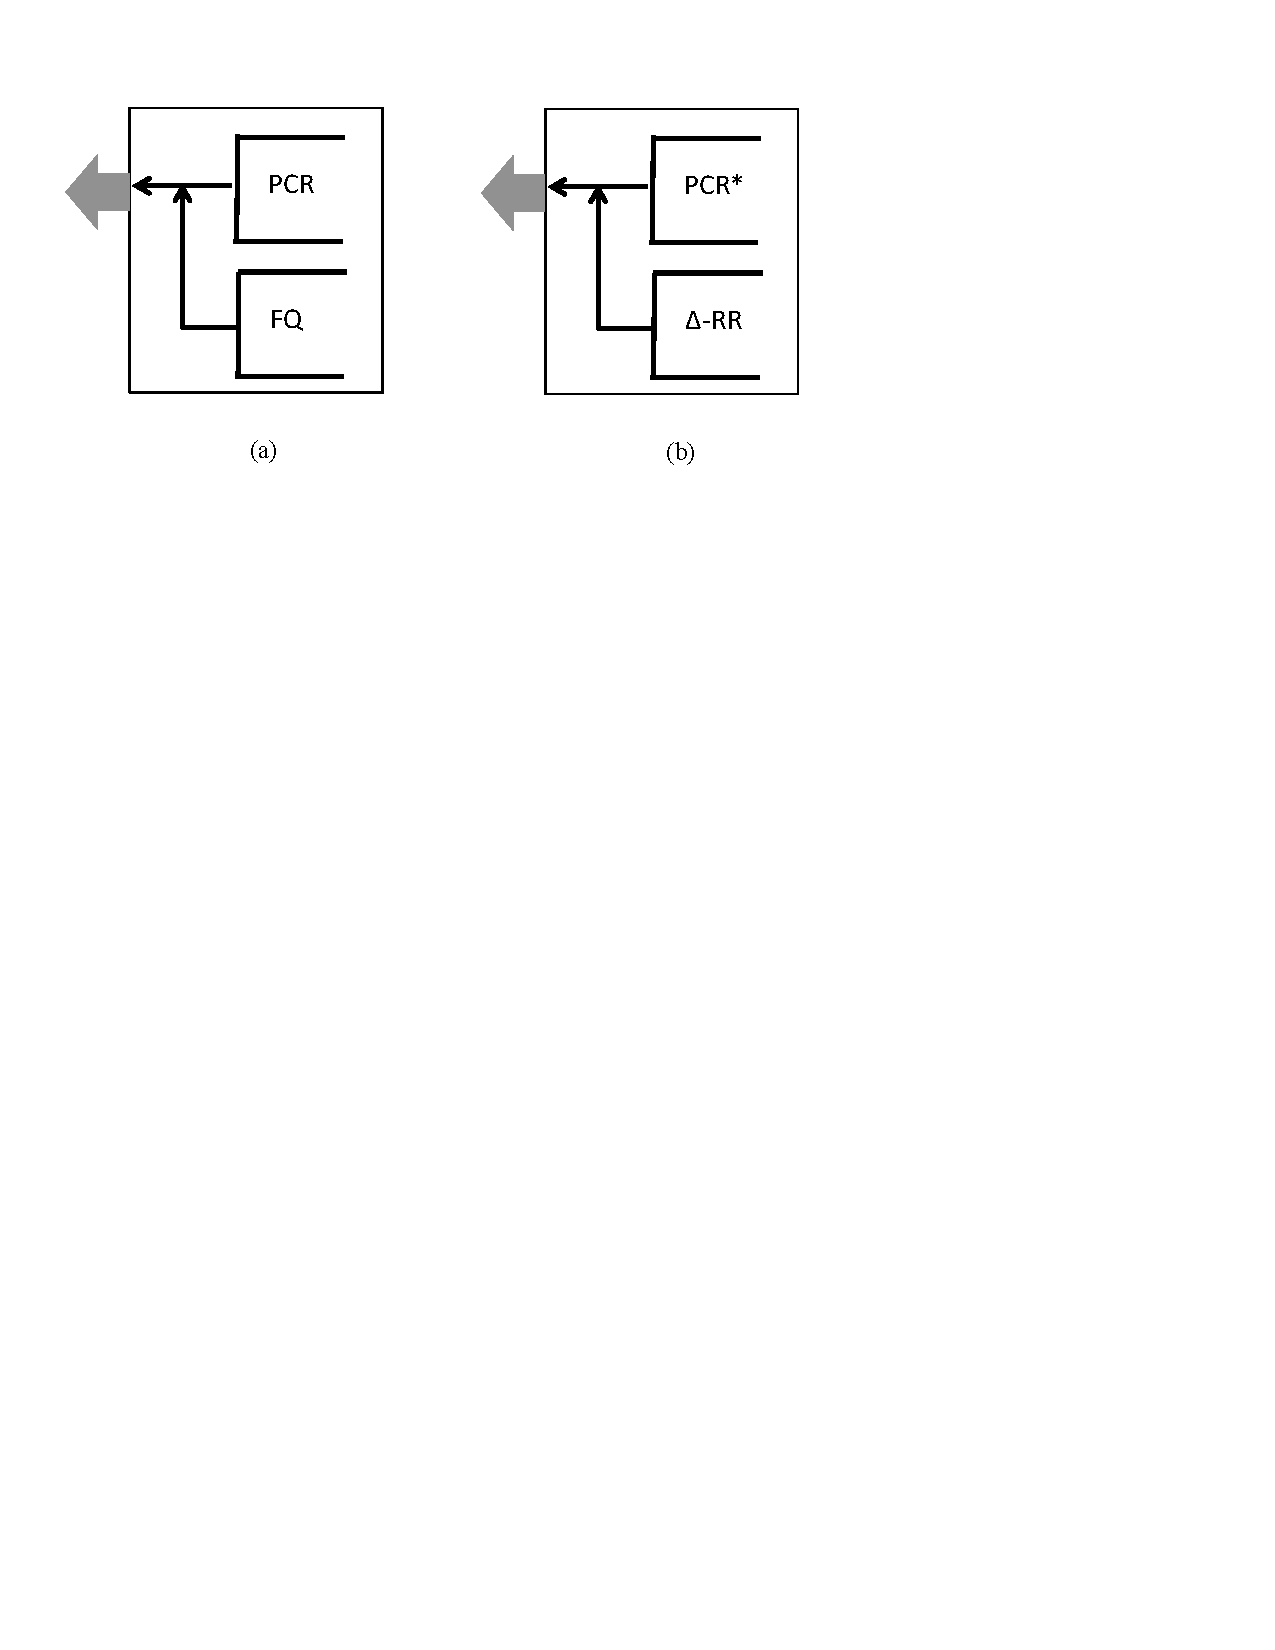
\includegraphics
[width=\columnwidth,trim=0.45in 7.9in 3.1in 0.7in,clip]
{FigDual.pdf}
}
\caption{Dual-Mode Scheduling}
\label{fig:Dual-Mode}
\end{figure}


\begin{figure}
\noindent
\rule{\columnwidth}{0.5mm}
\centerline{\bf PCR Scheduler}
\begin{tabbing}
\settabs
%Let $B(t)$ be the set of backlogged flows at time $t$.\\
upon receiving a packet $p_{f,i}$,\\
%\tea $S_{f,i,CR} = \mbox{max}(A_{f,i},F_{f,i,CR})$;\\
\tea $D_{f,i,PCR} = F_{f,i,CR}$;\\
\\
if output channel is idle at time $t$,\\
\tea let $p_{f,i} \in \mbox{Active}(t)$ iff $t \geq S_{f,i,CR}$;\\
\tea if $\mbox{Active}(t) \neq \emptyset$ then\\
\teb let $D_{g,j,PCR} = \mbox{min}\{D_{f,i,PCR}\,\,|\,\, p_{f,i} \in 
\mbox{Active}(t)\}$;\\
\teb forward $p_{g,j}$ to the output channel.  \end{tabbing}
\caption{Packetized constant-rate scheduler}
\label{fig:PCR}
\rule{\columnwidth}{0.5mm}
\end{figure}




Consider Figure \ref{fig:Dual-Mode}(a). The service required for an unenhanced 
flow $f$ is simply a constant rate $R_f$. This is provided by a packetized 
constant rate scheduler (PCR), which is described in more detail in Figure 
\ref{fig:PCR}. It is similat to the Virtual Clock protocol \cite{VC-Lam}, 
except that it does not allow flows to exceed their reserved rate. Note that 
this scheduler is non-work-conserving, i.e., there are times when its queues 
are non-empty yet it does not have any packets considered 'active', so it 
remains idle. Enhanced flows, on the other hand, have to be served in an equal 
manner.  This is best accomplished by a fair-queuing (FQ) scheduler, also shown 
in Figure \ref{fig:Dual-Mode}(a).

We thus have two schedulers, one for each type of flow. Priority is given to 
the PCR scheduler. I.e., when the output channel becomes idle, the PCR 
scheduler is queried for the next packet to be transmitted. Only if the PCR 
scheduler is unable to provide a packet (due to its queues being empty or all 
packets being 'inactive'), then the packet transmitted is chosen from the FQ 
scheduler. Both of these schedulers can be implemented in $O(\log(n))$ time per 
packet arrival/departure (FQ using the method of \cite{WFQlogN}).

The above method should work, provided the membership in the enhanced and 
unenhanced flow sets remains constant. However, their membership depends on 
unallocated bandwidth. An increase in unallocated bandwidth enhances more 
flows, and a decrease unenhances some flows. 

Unallocated bandwidth comes from two sources: from bandwidth that is not 
reserved by any flow, and from flows that have temporarilly stopped creating 
packets (empty queues). The former is relatively stable, and changes are 
predictable (when flows are added or removed). In this case, the appropriate 
movement of flows between the schedulers can be done before a new flow is 
accepted or removed from the system. The latter, i.e., queues becoming empty, 
cannot be predicted, and may cause large changes in flow assignments to the two 
schedulers. This is particularly true if the flows whose queue becomes empty 
have a large reserved bandwidth. Thus, moving flows from one scheduler to the 
other is not efficient, which prompts us to present below our final version of 
the scheduler.


%%%%%%%%%%%%%%%%%%%%%%%%%%%%%%%%%%
\subsection{Static-Flow-Assignment Scheduler}
%%%%%%%%%%%%%%%%%%%%%%%%%%%%%%%%%
\label{subsec:Static-Flow-Scheduler}


\begin{figure}
\noindent
\rule{\columnwidth}{0.5mm}
\centerline{\bf A-PEQ Scheduler}
\begin{tabbing}
\settabs
upon receiving a packet $p_{f,i}$,\\
\tea add $p_{f,i}$ to the queue of $f$, $Q_f$;\\
\\
if output channel is idle at time $t$,\\
\tea model the behavior of $\femph{PCR}$ to dequeue a packet;\\
\tea let $p_{f,i}$ be the packet chosen by $\femph{PCR}$;\\
\tea let $\rho_{min} = \mbox{min}\{\rho_g \,\,|\,\, Q_g \neq \emptyset\}$;\\
\tea if $Q_f \neq \emptyset$ then\\
\teb    dequeue and forward a packet from flow $f$;\\
\teb    $\rho_f = \mbox{min}(\rho_f+1,\rho_{min}+\Delta)$;\\
\tea else\\
\teb    let $g$ satisfy $\rho_g = \rho_{min}$;\\
\teb    forward the next packet of flow $g$;\\
\teb    $\rho_g = \rho_g + 1$;\\


\end{tabbing}
\caption{Approximate packetized rate equalization scheduler}
\label{fig:A-PEQ-Scheduler}
\rule{\columnwidth}{0.5mm}
\end{figure}




Our final protocol, {\em Approximate Packetized rate Equalization} (A-PEQ), is 
shown in detail in Figure \ref{fig:A-PEQ-Scheduler}, with an abstract view in 
Figure \ref{fig:Dual-Mode}(b). For this implementation, we make the simplifying 
assumption that all packets of all flows have an equal size, L.\footnote{We 
will investigate eliminating this restriction in future work.} There are three 
major differences from the previous scheduler.

First, {\em all flows take part in both schedulers}. This solves the problem of 
having to move a large number of flows between the schedulers in a short period 
of time. 

Second, the scheduler PCR* differs from PCR as follows. PCR* assumes that every 
flow always has packets available (even if its queue is empty). When it chooses 
a packet from flow $f$ for transmission, it checks the queue of $f$. If it is 
empty, then the packet transmitted is instead a packet chosen by $\Delta$-RR.  
Eventhough $f$ did not transmit a packet, PCR* updates its state about $f$ as 
if indeed it had transmitted a packet from $f$.  

Third, instead of FQ, we have a modified round-robin scheduling, which we 
denote $\Delta$-RR. Each flow $f$ has a round number $\rho_f$ in $\Delta$-RR.  
When $\Delta$-RR is asked to forward a packet, it chooses it as follows.

\begin{itemize}
\item
If $\Delta$-RR is called because PCR* is unable to transmit a packet, then 
$\Delta$-RR chooses a packet from the backlogged flow {\em with the least 
round-number}, and increases the flow's round number by one.
\item
If PCR* is able to transmit a packet from a flow $f$, then the round-number of 
$f$ is increased by one, {\em even though} $\Delta$-RR {\em did not output a 
packet}.
\end{itemize}

The motivation for the above choices is as follows. Consider two flows $f$ and 
$g$, where $f$ has a large reserved rate (always unenhanced in the fluid 
server) and $g$ a small reserved rate (always enhanced in the fluid server).  
All unenhanced flows, such as $f$, transmit packets from PCR* at a high rate, 
so their round numbers in $\Delta$-RR are higher than those of other flows.  
The slower flows, such as $g$, are served in round-robin order, and thus 
receive the same bandwidth. 

Consider now two slow flows $g$ and $h$, with $g$ having a greater reserved 
rate than $h$.  Note that through their respective packet transmissions at 
PCR*, the round number of $g$ grows faster than $h$'s. Nonetheless, both flows 
receive about the same behavior from $\Delta$-RR. This is because the unused 
bandwidth at PCR* causes $\Delta$-RR to serve the slowest flows, such as $h$, 
first, which allows these flows to reach the same round numbers as other flows, 
such as $g$.


One final detail remains. Assume the round number of flow $f$, due to its large 
reserved rate, grows much larger than that of other flows. Then, assume enough 
bandwidth becomes available to make $f$ an enhanced flow in the fluid server.  
However, due its large round number, $f$ will not receive service in 
$\Delta$-RR for a long time.  To avoid this, we place a bound, $\Delta$, on the 
difference between the round number of any flow and the minimum round number of 
any backlogged flow, as indicated in Figure \ref{fig:A-PEQ-Scheduler}. 

The bound $\Delta$ is a tunable parameter of the system. If it is too large, 
enhanced flows may not receive their due bandwith, and if it is too small, 
bandwidth may be wasted on unenhanced flows. 

%%%%%%%%%%%%%%%%%%%%%%%%%%%%%%%%%%%%%%%%%%%%%%%%%%%%%%%%%%%%%%%%
%
\section{Future Work and Concluding Remarks}
\label{sec: future work}
%
%%%%%%%%%%%%%%%%%%%%%%%%%%%%%%%%%%%%%%%%%%%%%%%%%%%%%%%%%%%%%%%%


{\em
Several directions for future work are possible. First, it is yet to be 
determined the tightness of the bound in Theorem \ref{thm: main}. Also, a 
smaller value of $\delta_{s,f,i}$ may be possible by using a technique similar 
to that in \cite{RP-Fair-Servers-ToN}, as follows. Each packet $p_{f,i}$ does 
not become ``available'' until its start time, $S_{s,f,i}$. The scheduler $s$ 
gives preference to available packets, and among these, it forwards the packet 
with the smallest deadline, $S_{s,f,i} + L_{f,i}/R_f$. If no packet is 
available, then the scheduler chooses packets in a form similar to the virtual 
rate-equalizing scheduler $\hat{s}$. The above will ensure $\delta_{s,f,i} = 
L_{f,i}/R_f + L^{max}_s/C_s$. However, it is not clear how this would affect 
the bound of Theorem \ref{thm: main}. 

The time complexity of en-queuing or de-queuing a packet in rate-equalization 
is $O(n)$, where $n$ is the number of flows. For a long time, it was believed 
that WFQ also had an $O(n)$ complexity. However, via sophisticated indexing 
techniques, a $O(\log(n))$ bound was obtained \cite{WFQlogN}. We will continue 
to study the complexity of rate-equalization and determine if a lower 
complexity implementation can be found.


Finally, scheduling packets over multiple parallel links between neighboring 
computers has been studied for guaranteed-rate schedulers 
\cite{Cobb-Multi-Channel-JHSN} \cite{Cobb-Multi-Channel-IWQoS} 
\cite{MPGPS-Ozden}. We also plan to investigate the impact of rate-equalization 
over parallel links.
}

\bibliographystyle{plain}
\bibliography{./IEEEabrv,./bibliography}

\end{document}



%%%%%%%%%%%%%%%%%%%
%%%%%%%%%%%%%%%%%%%
%%%%%%%%%%%%%%%%%%%
%%%%%%%%%%%%%%%%%%%
%%%%%%%%%%%%%%%%%%%
%%%%%%%%%%%%%%%%%%%
%%%%%%%%%%%%%%%%%%%
%%%%%%%%%%%%%%%%%%%
%%%%%%%%%%%%%%%%%%%
\begin{tabular}{ll}
{\bf Notation}\\
Constant Rate fluid server & CR\\
non-conserving Packetized CR & PCR (i.e., VC2)\\
EQualization fluid server & EQ\\
Packetized EQualization scheduler & PEQ\\
%Packetized CR & VC  \\
Approximate PEQ  & A-PEQ\\
{\bf Rate Guaranteed} \\
start time & $S_{f,i,CR}$\\
finish time & $F_{f,i,CR}$\\
{\bf Flow always with packets}\\
(for APREQ, when xmitting $\femph{f}$\\
 pick a packet from $f$, if none, then \\
 go to round-robin schedule) \\
start time & $S_{\femph{f},i,CR}$\\
finish time & $F_{\femph{f},i,CR}$\\
{\bf Deadlines for Packet }\\
{\bf schedulers }\\
$D_{f,i,PEQ}$ & $S_{f,i,EQ} + L/R_f$\\
$D_{f,i,A-PEQ}$ & $S_{\femph{f},k,CR} + L/R_f$\\
where $k$ is the next packet \\
of $\femph{f}$ when $p_{f,i}$ \\
reaches the head of its \\
queue.
\end{tabular}


